\begin{question}
\noindent A space agency designs a scale model of a satellite dish support frame, shown as shape $M$ on the grid below. The full-size frame will be built by enlarging the model with a centre of enlargement at point $(-6,6)$ and a scale factor of $\dfrac{1}{2}$.

\begin{center}
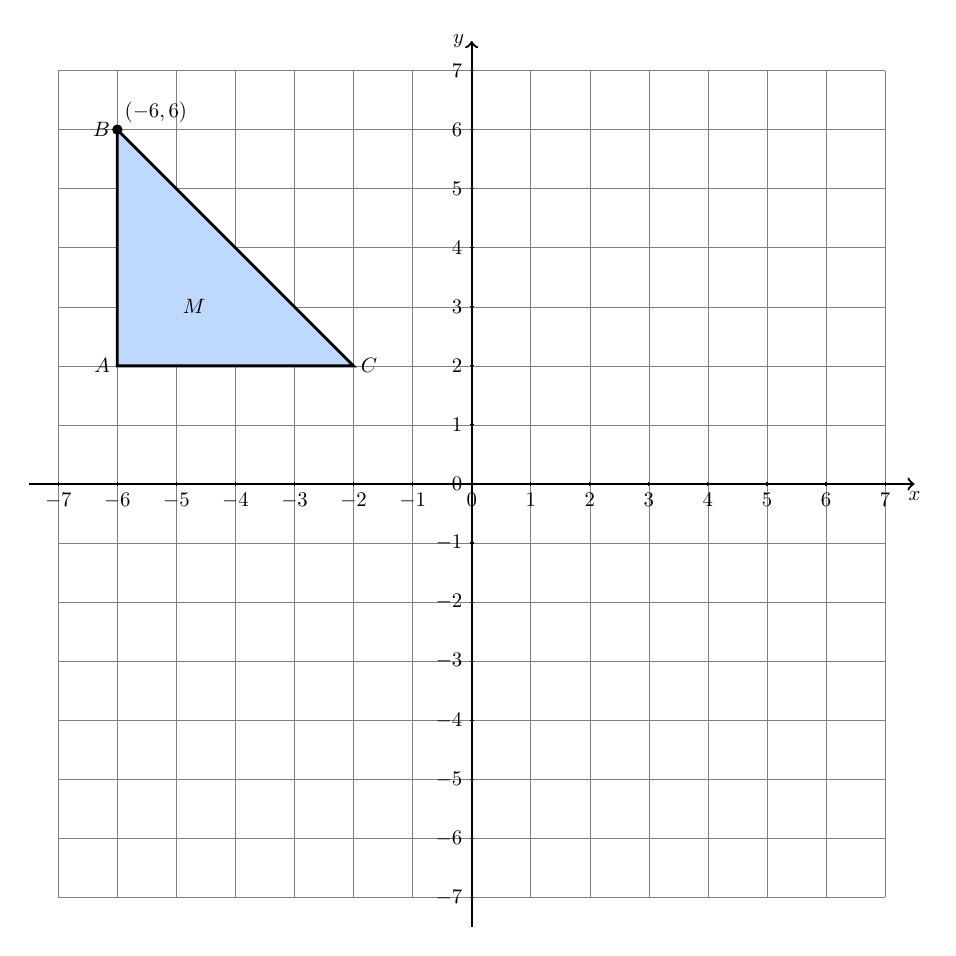
\begin{tikzpicture}[scale=0.75, transform shape]
    \def\axisLimit{7}

    \definecolor{borderColour}{HTML}{000000}
    \definecolor{fillColourM}{HTML}{BFD8FF}

    % Draw grid
    \draw[step=1cm,gray,very thin] (-\axisLimit,-\axisLimit) grid (\axisLimit,\axisLimit);

    % Draw axes
    \draw[thick,->] (-\axisLimit-0.5,0) -- (\axisLimit+0.5,0) node[anchor=north] {$x$};
    \draw[thick,->] (0,-\axisLimit-0.5) -- (0,\axisLimit+0.5) node[anchor=east] {$y$};

    % Label x-axis and y-axis
    \foreach \x in {-\axisLimit,...,\axisLimit}
        \draw (\x cm,1pt) -- (\x cm,-1pt) node[anchor=north] {$\x$};
    \foreach \y in {-\axisLimit,...,\axisLimit}
        \draw (1pt,\y cm) -- (-1pt,\y cm) node[anchor=east] {$\y$};

    % Shape M: vertices A(-6,2), B(-6,6), C(-2,2)
    \coordinate (A) at (-6,2);
    \coordinate (B) at (-6,6);
    \coordinate (C) at (-2,2);
    \filldraw[fill=fillColourM, draw=borderColour, line width=1pt] (A) -- (B) -- (C) -- cycle;

    \node[left] at (A) {$A$};
    \node[left] at (B) {$B$};
    \node[right] at (C) {$C$};
    \node at (-4.7,3) {$M$};

    % Centre of enlargement
    \coordinate (centre) at (-6,6);
    \fill[black] (centre) circle (2.5pt);
    \node[above right] at (centre) {$(-6,6)$};

\end{tikzpicture}
\end{center}

\noindent On a copy of the grid, draw the image of shape $M$ after an enlargement with scale factor $\dfrac{1}{2}$ and centre of enlargement $(-6,6)$.\\
Label the image $M'$.

\vspace{4.5cm}

\begin{flushright}
\answerlines{4}{3}
\end{flushright}
\end{question}
